\documentclass[a4paper, 12pt]{article}
\usepackage{amsmath}
\usepackage{amsthm}
\usepackage{amssymb}
\usepackage{longtable}
\usepackage{pdflscape}
\usepackage{algorithm}
\usepackage{graphicx}
\usepackage[noend]{algpseudocode}
\usepackage{url}
\usepackage{tikz}
\usetikzlibrary{arrows}
\usepackage{float}

\newlength\tindent
\setlength{\tindent}{\parindent}
\setlength{\parindent}{0pt}
\renewcommand{\indent}{\hspace*{\tindent}}

\newtheorem{thm}{Theorem}
\newtheorem{cor}{Corollary}[thm]
\newtheorem{lemma}{Lemma}[thm]

\title{NWEN 303 Assignment 1}
\author{Daniel Braithwaite}

\begin{document}
	\pagenumbering{gobble}
	\maketitle
	\newpage
  	\pagenumbering{arabic}
  	
	\section{Synchronization}
		\subsection{Part a}
			A race condition occurs when the order of execution of threads can effect the outcome. In the given example we have two race conditions one with the variable k and the other with the variable found. Now we discuss the behavior these race conditions can cause
			
			\begin{enumerate}
				\item \textbf{Variable K:} The issue here is that each of the threads is overwriting the variable k. Say we start the first thread with i as 0 and then start the thread with i as 1. The first thread sets k to be 0. and then before the first loop gets to check if $f(0) = 0$ the second thread comes along and sets k to 1 so we never get to check $f(0)$. Along with this we have that each thread is constantly updating k to be $k + N$. This results in a lot of numbers being skipped.
				
				\item \textbf{Variable found:} This race condition can cause threads to run to run longer than they should. If one thread finds a number k satisfying $f(k) = 0$ then it will update the found variable to be true. But if before the variable can be updated another thread finds a way to satisfy the equation then two numbers will be printed out where we only want one.
			\end{enumerate}
			
			
		\subsection{Part b}
			An easy way to solve the issues caused by the race condition with the variable k is to have each thread store a local variable k. There is no reason for the threads to be sharing the variable in the first place.\\
			
			If there is multiple values k that give $f(k) = 0$ and we only want to print out the first one that gets found. We allow any thread to read the found variable but if a thread finds a solution it must acquire a lock before it can update found and print out the solution. After a thread acquires a lock it checks to see if found is set to true if it is then we already have a solution and can exit. 
			
			We can implement both these solutions without getting a deadlock as there is only one shared resource.
			
		\subsection{Part c}
			Fairness refers to the scheduler ensuring all threads are able to run for the same amount of time. If we don't have fairness then we can end up with a large chunk of the function domain not being tested because the thread responsible for testing them isn't being run.
			
		\subsection{Part d}
			You could create some object that handles giving out values of k to be tested. Then each thread will ask this object for the a number, test the number and repeat. While doing this would work in the absence of fairness it would make the object allocating the numbers a point of contention significantly reducing the performance given that all the threads are regularly trying to access this object. How ever if the algorithm for computing $f$ is slow then this using this solution could still be efficient.
			
	\section{Measuring Array Sum}
		I experimented with the array sizes by starting from 100 and increasing by multiples of 10, for each array size I would run the sum with no threads and then with 0 to 50 threads to get a better picture of the performance trend. Each test was averaged over 70 runs. Until the array sizes get to 100000 or 1000000 the threading doesn't seem to have any effect on the sum time of the array (there are some fluctuation but nothing consistent), adding the threading only adds the overhead of creating the threads which ends up just slowing the summing down.
		
		\begin{figure}[H]
			\minipage{0.32\textwidth}
  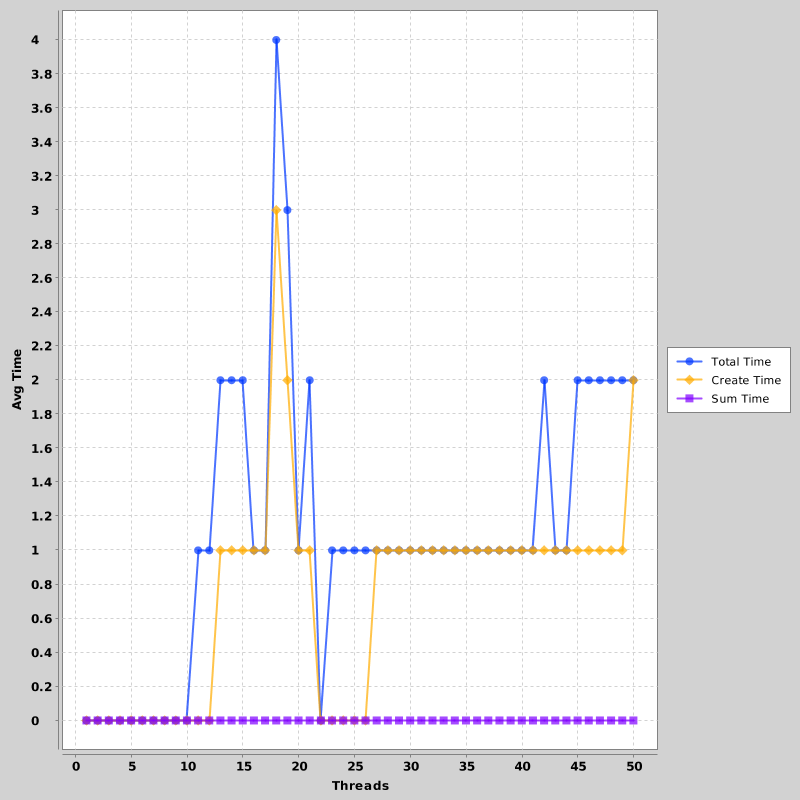
\includegraphics[width=\linewidth]{threads-vs-time-100-global.png}
  \caption{Array size of 100. Time taken with no threads is 0ms}
\endminipage\hfill
\minipage{0.32\textwidth}
  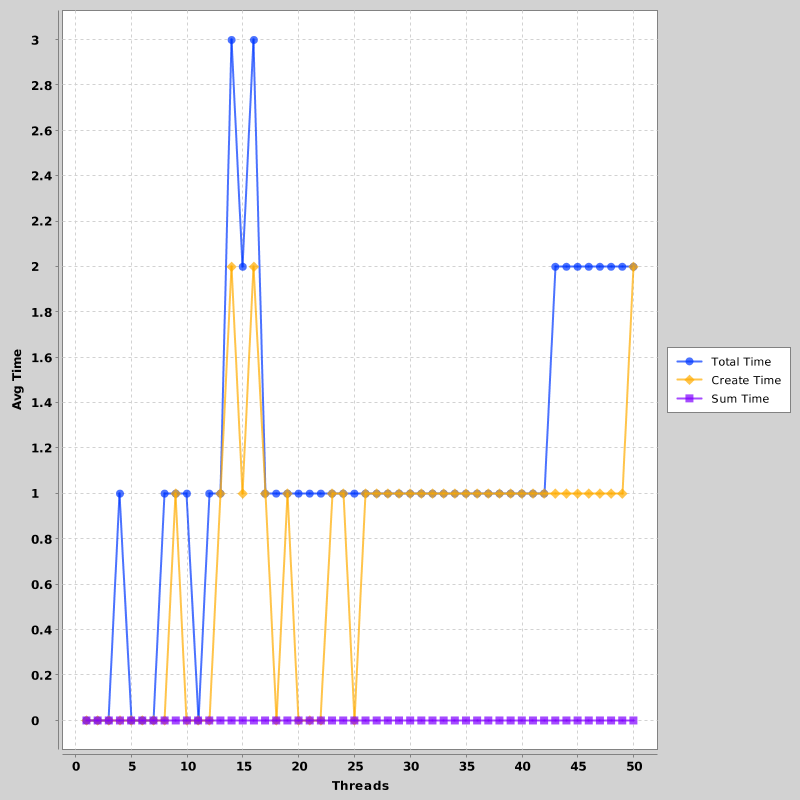
\includegraphics[width=\linewidth]{threads-vs-time-1000-global.png}
  \caption{Array size of 1000. Time taken with no threads is 0ms}
\endminipage\hfill
\minipage{0.32\textwidth}%
  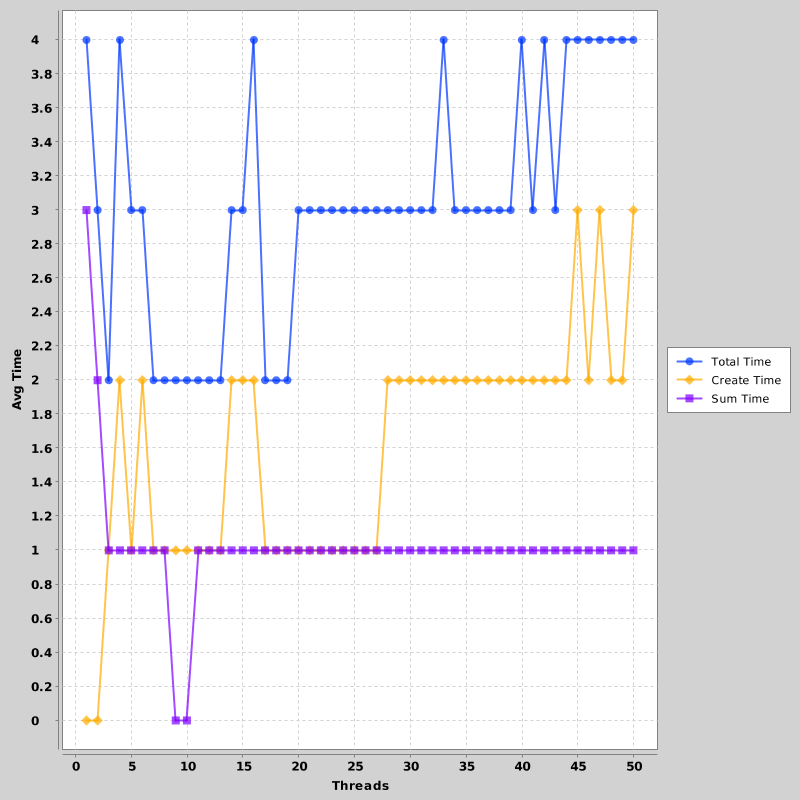
\includegraphics[width=\linewidth]{threads-vs-time-10000-global.png}
  \caption{Array size of 10000. Time taken with no threads is 0ms}
\endminipage
		\end{figure}
		
		\newpage
		
		On average it takes 0ms to sum 100000 elements with no threads so you would expect that when summing using only 1 thread the total sum time would be the same how ever the opposite was true it was 28ms.\\
		
		After each thread added a number to the global sum it would call its yeald method, telling the scheduler that the thread was willing to give up the rest of its time slice. The problem with using this yeald so frequently is that the operation of pausing a currently running thread and starting another is expensive.\\	
		
		After disabling the $this.yeald()$ statement in the thread the performance significantly improved.
		
		
				\begin{figure}[H]
			\minipage{0.48\textwidth}
  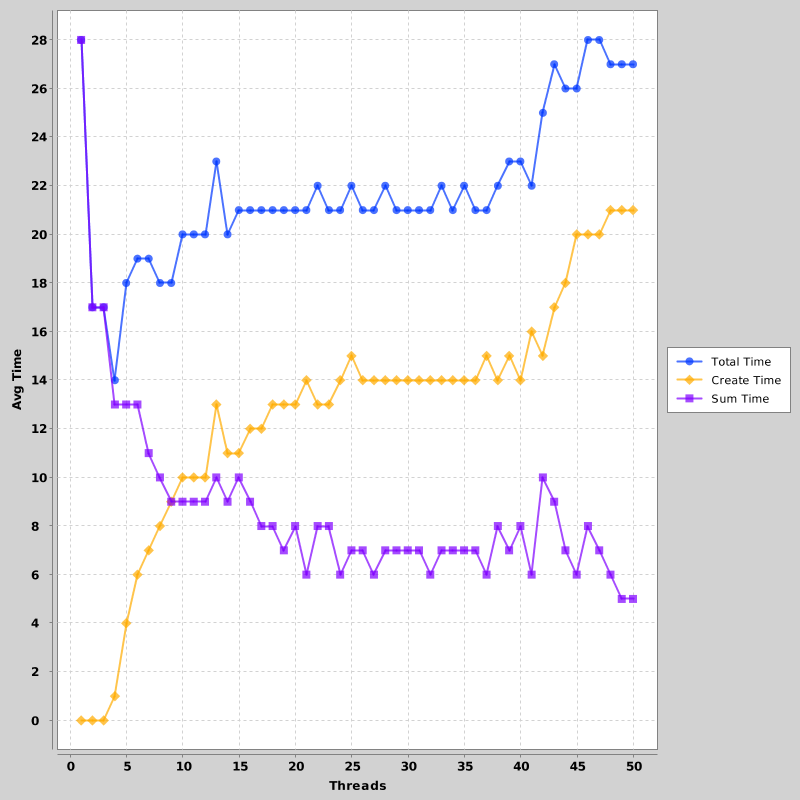
\includegraphics[width=\linewidth]{threads-vs-time-100000-global.png}
  \caption{Summing 100000 elements with yeald}
\endminipage\hfill
\minipage{0.48\textwidth}
  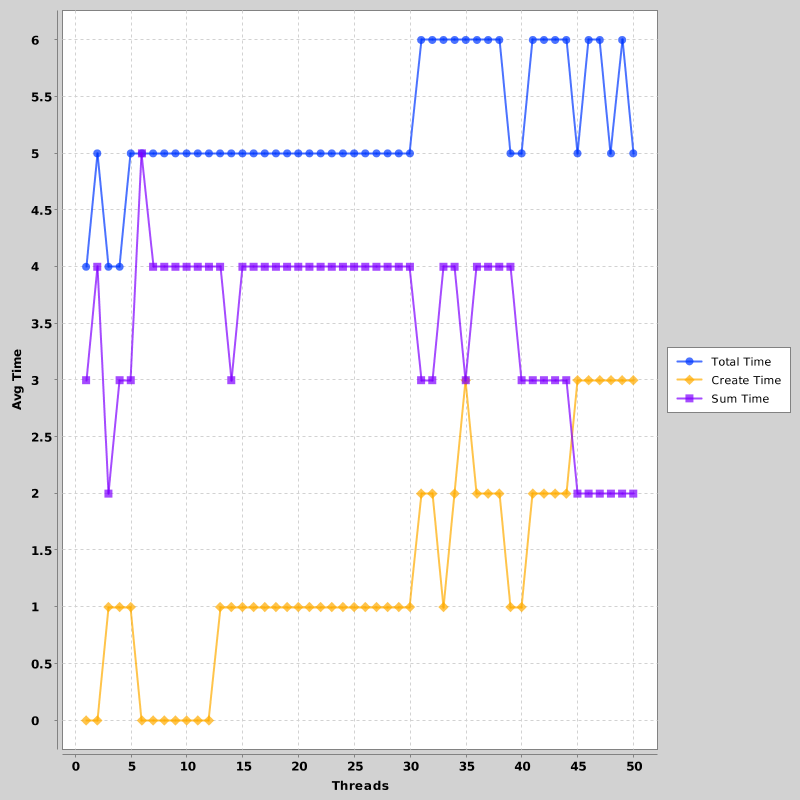
\includegraphics[width=\linewidth]{threads-vs-time-100000-global-noyield.png}
  \caption{Summing 100000 elements without yeald}
\endminipage\hfill
		\end{figure}		
	
		However even with this removed there is still a discrepancy between the time taken with running the sum on a single new thread as opposed to running the sum on just the main.main thread (we would expect the times to be the same as the creation time of 1 thread is negligible). The sum time displayed in the graph is determined by recording how long it takes to join with all the threads, indicating that there is some other overhead.\\
		
		So far we have been summing everything directly to the global sum variable, causing a lot of contention as all the threads are trying to access this one variable. Another option is to use a local sum variable on each of the threads so that each thread uses its local sum and only once a thread has finished summing will it add to the global sum.\\
		
		\newpage
					
		\begin{figure}[H]
			\minipage{0.48\textwidth}
  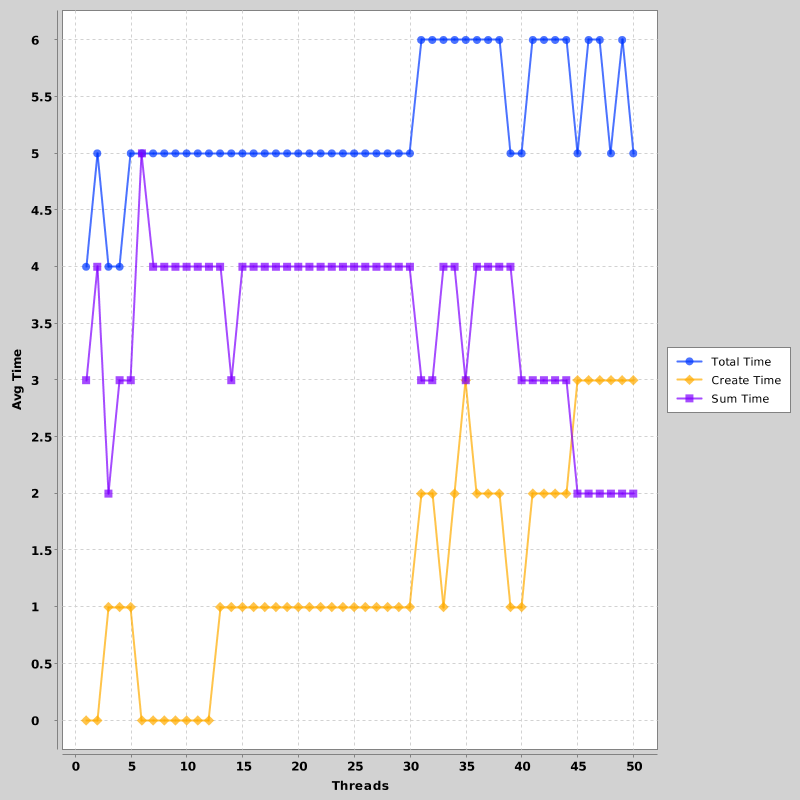
\includegraphics[width=\linewidth]{threads-vs-time-100000-global-noyield.png}
  \caption{Summing 100000 elements without yeald and with all threads adding to the global sum}
\endminipage\hfill \minipage{0.48\textwidth}
  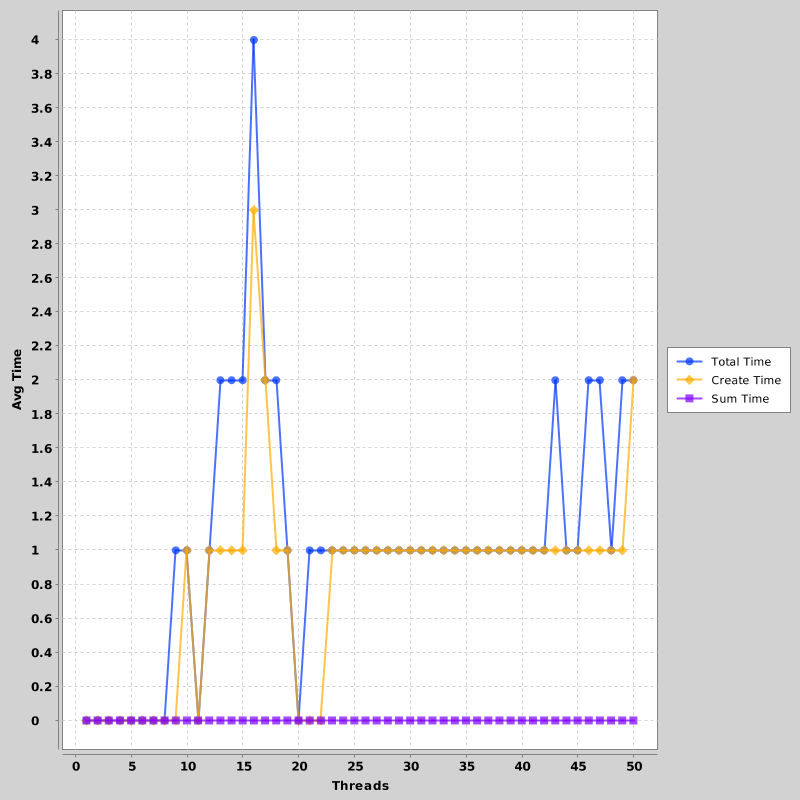
\includegraphics[width=\linewidth]{threads-vs-time-100000-local-noyield.png}
  \caption{Summing 100000 elements without yeald with each thread summing to a local sum variable first}
\endminipage\hfill
		\end{figure}		
	
		Comparing the two graphs we see that the use of a local sum has removed the extra overhead we saw before. Now the summing of each thread is just as quick as summing with no threads. How ever the overhead is still causing this method to be less efficient. Now that our program is a lot faster we can increase the number of elements in our array. The largest array size my computer could handle was 10000000 (Any larger ether caused an out of memory exception or froze my computer).
		
		
		\begin{figure}[H]
  			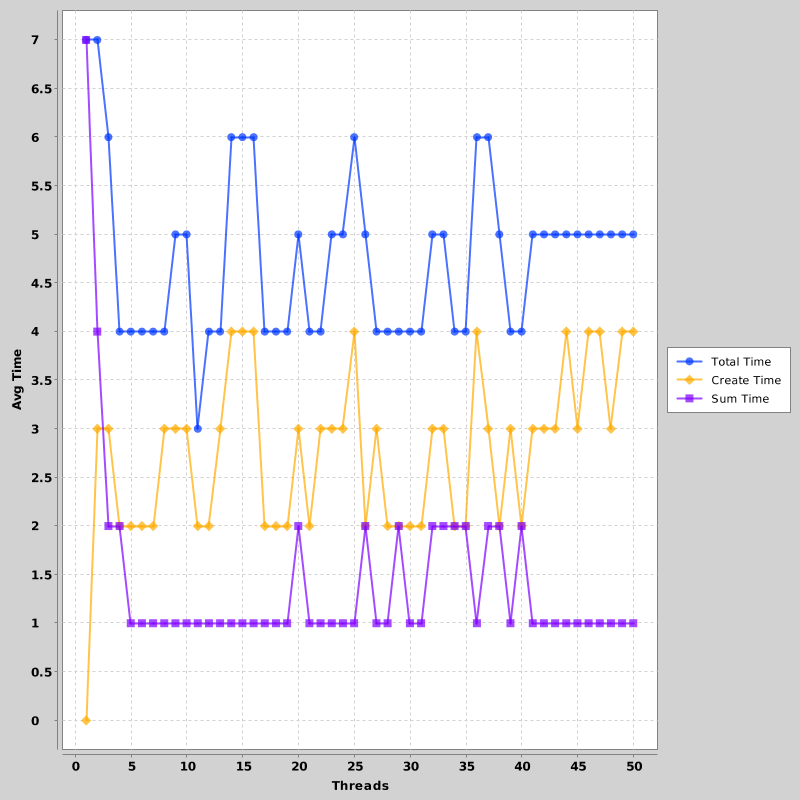
\includegraphics[scale=0.5]{threads-vs-time-10000000-laptop.png}
  			\caption{Summing 10000000 with local sum variable and no yeald. Using no threading took 6ms}\hfill
		\end{figure}
		
		The results of this run where promising as the multi threaded solution usually ether performed just as well or better than using no threads. Now we can compare the performance of running this algorithm on different computers.
		
		\begin{figure}[H]
			\minipage{0.48\textwidth}
  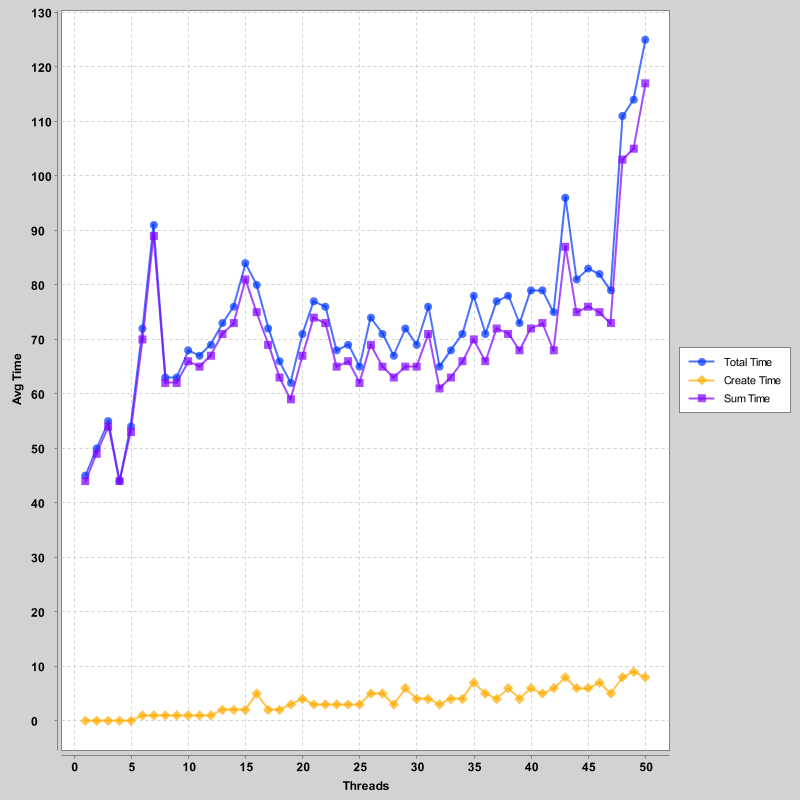
\includegraphics[width=\linewidth]{threads-vs-time-10000000-anna.png}
  \caption{Home PC 1, Array size of 10000000. Time taken with no threading 19ms}
\endminipage\hfill
\minipage{0.48\textwidth}
  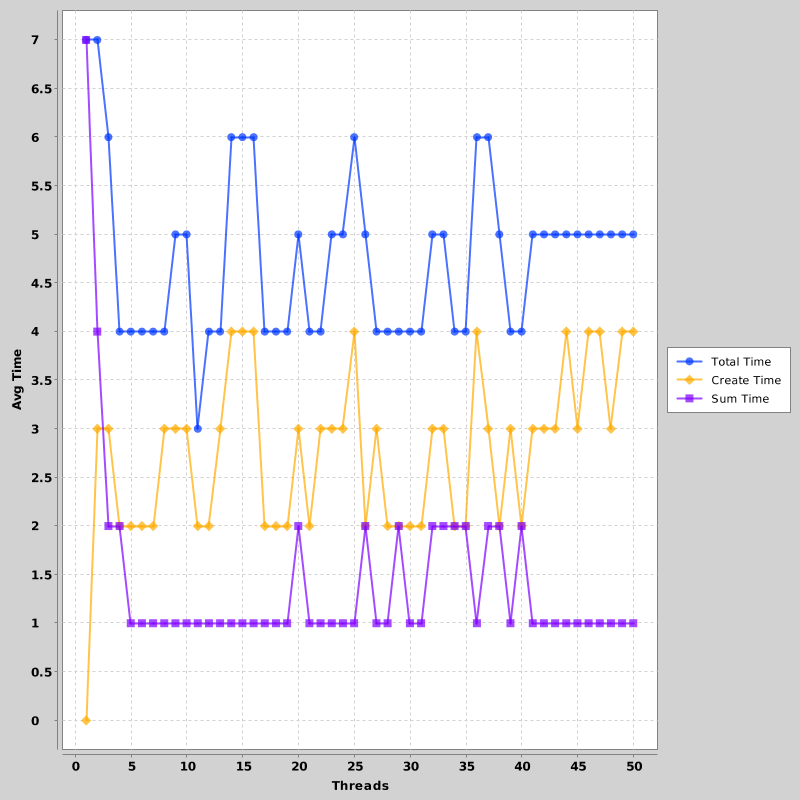
\includegraphics[width=\linewidth]{threads-vs-time-10000000-laptop.png}
  \caption{Home Laptop, Array size of 10000000, Time taken with no threading 6ms}
\endminipage\hfill
		\end{figure}
		
		\begin{figure}[!htb]
\minipage{0.48\textwidth}%
  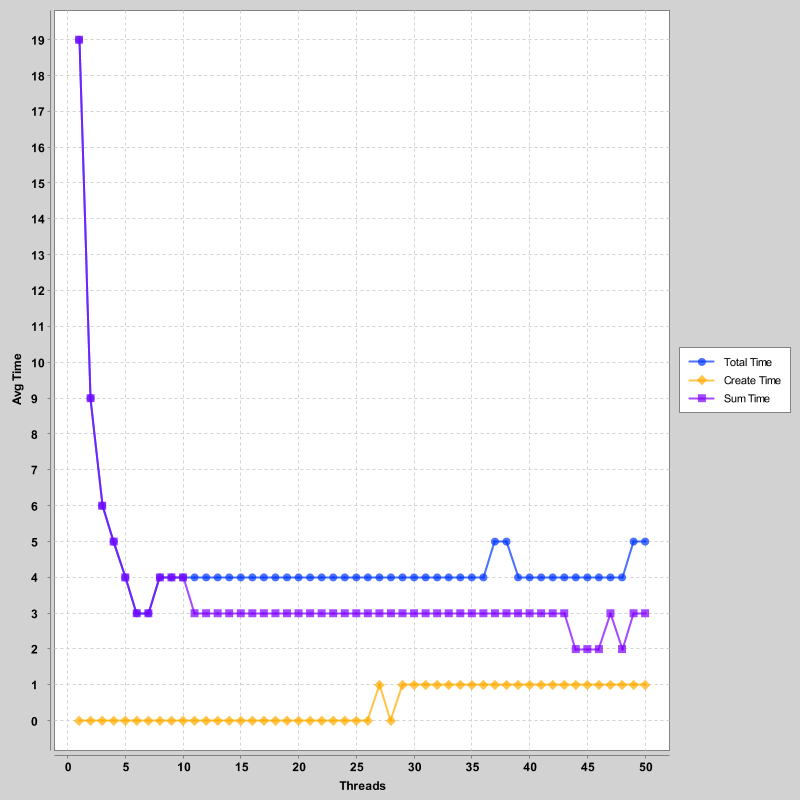
\includegraphics[width=\linewidth]{threads-vs-time-10000000-desktop.png}
  \caption{Home PC 2, Array size of 10000000, Time taken with no threading 5ms}
\endminipage\hfill
\minipage{0.48\textwidth}%
  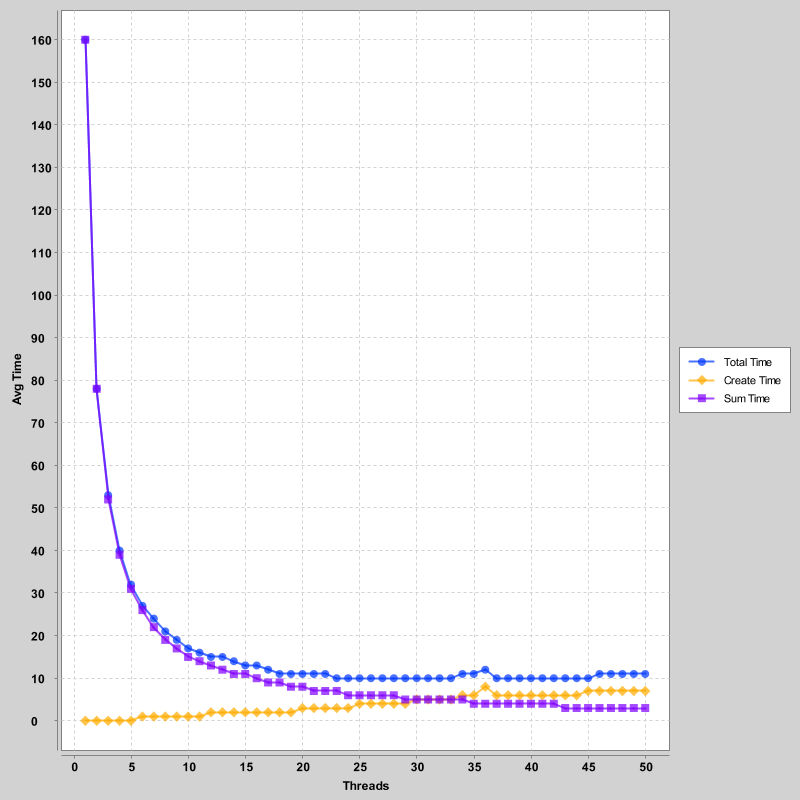
\includegraphics[width=\linewidth]{threads-vs-time-10000000-lighthouse.png}
  \caption{Lighthouse, Array size of 10000000, Time taken with no threading 157ms. NOTE: only included up to 50 threads as going up to 64 didn't appear to have any improvement}
\endminipage\hfill
		\end{figure}		
		
		
		\begin{enumerate}
			\item \textbf{Home PC 1:} Has 1 core, and 1 thread per core. Total of 1 CPU's running at 2.7GHz
			
			\item \textbf{Home Laptop:} Has 2 cores, and 2 threads per core. Total of 4 CPU's running at 1.6GHz
			
			\item \textbf{Home PC 2:} Has 4 cores, and 2 threads per core. Total of 8 CPU's running at 3.5GHz
			
			\item \textbf{Lighthouse:} Has 64 CPU's
		\end{enumerate}
	
		As you would expect the multi threaded sum performs awfully on Home PC 1 as there is only one core to run each of the threads on, so you cant have threads running in parallel. Home PC 2 and Home Laptop show some improvement from summing with no threads but there aren't enough CPU's to run all the threads so the overhead of the multi threading means there is no significant improvement. Finally Lighthouse gets a significant performance increase as the bulk number of CPU's allows us to run lots of threads at once.\\
		
		From the above discussion I would conclude that there is no benefit to solving this problem using multi threading unless you know you are going to be running your program on a machine like Lighthouse.
	
	\newpage	
	
		
	\section{Recursive Array Sum}
		Using the same 4 computers as before we can try different threshold values to find an optimal value.
		
				\begin{figure}[H]
			\minipage{0.48\textwidth}
  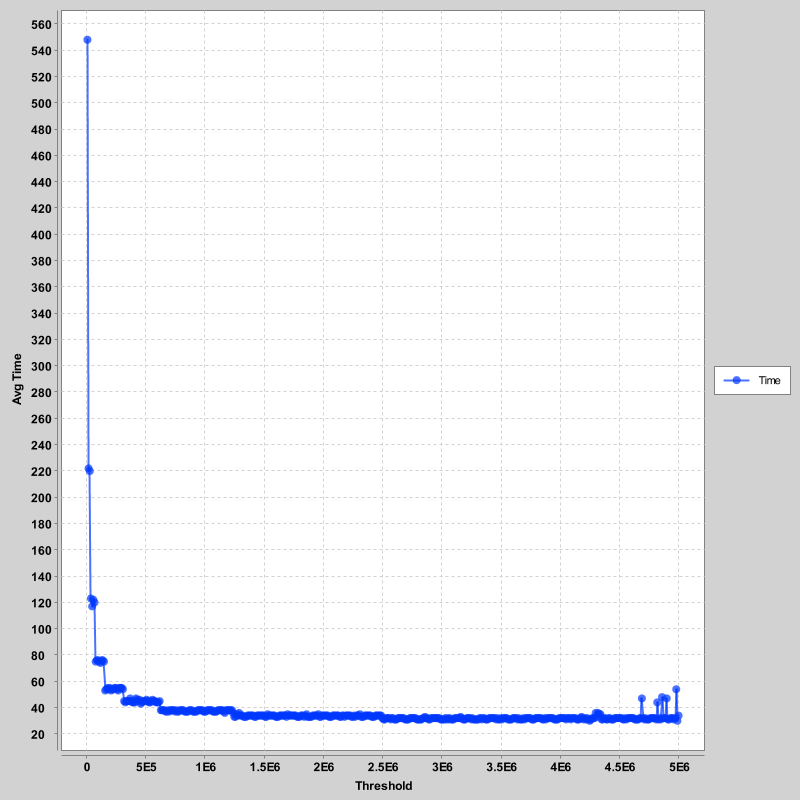
\includegraphics[width=\linewidth]{thres-vs-time-pc-1.png}
  \caption{Home PC 1, Array size of 10000000. Time taken with no threadding 19ms}
\endminipage\hfill
\minipage{0.48\textwidth}
  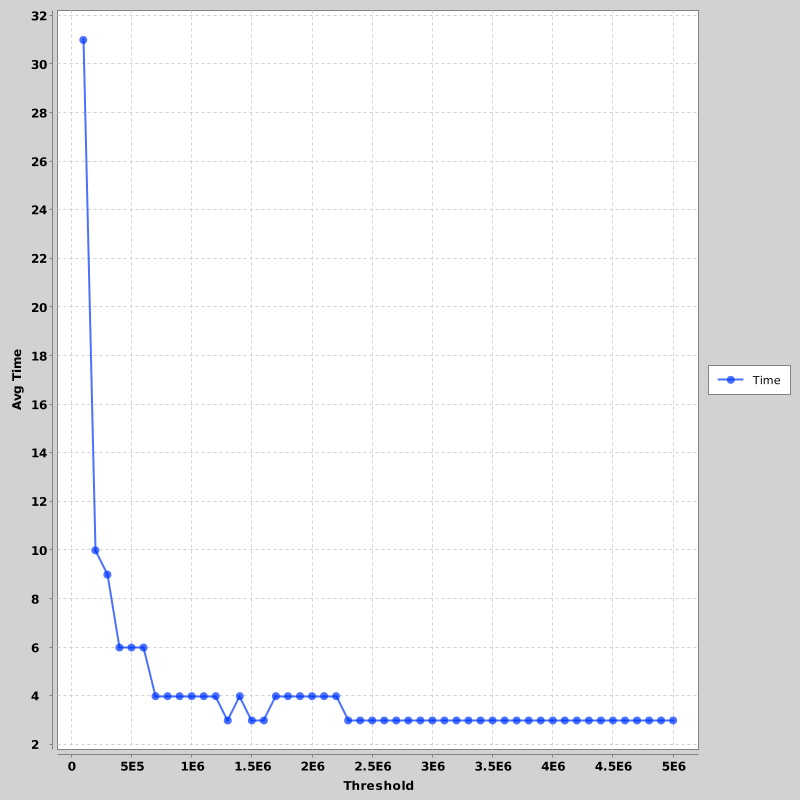
\includegraphics[width=\linewidth]{thres-vs-time-laptop.png}
  \caption{Home Laptop, Array size of 10000000, Time taken with no threading 6ms}
\endminipage\hfill
		\end{figure}
		
		\begin{figure}[H]
\minipage{0.48\textwidth}%
  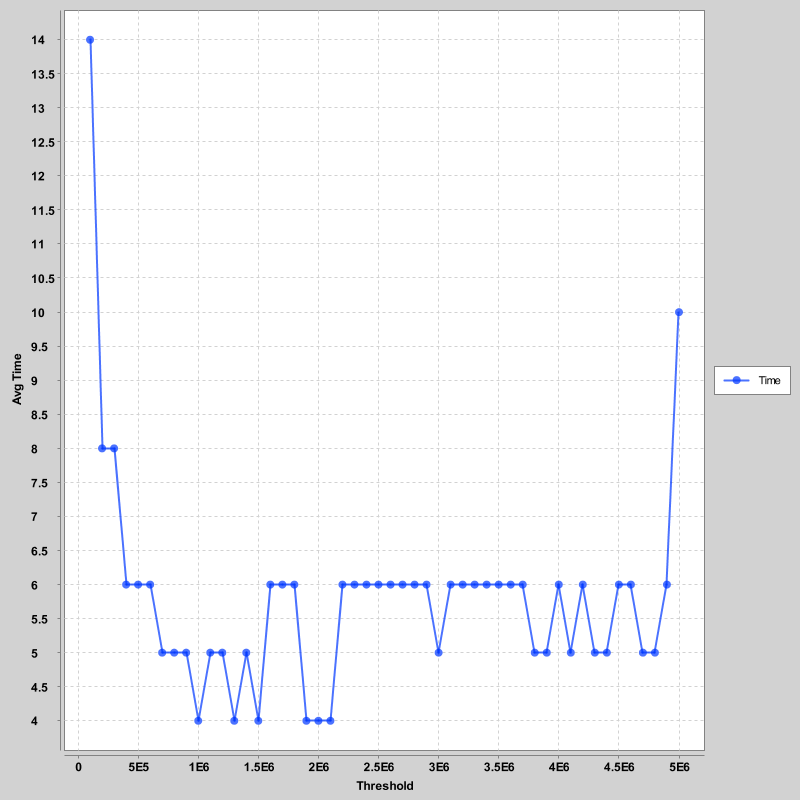
\includegraphics[width=\linewidth]{thres-vs-time-pc-2.png}
  \caption{Home PC 2, Array size of 10000000, Time taken with no threading 5ms}
\endminipage\hfill
\minipage{0.48\textwidth}%
  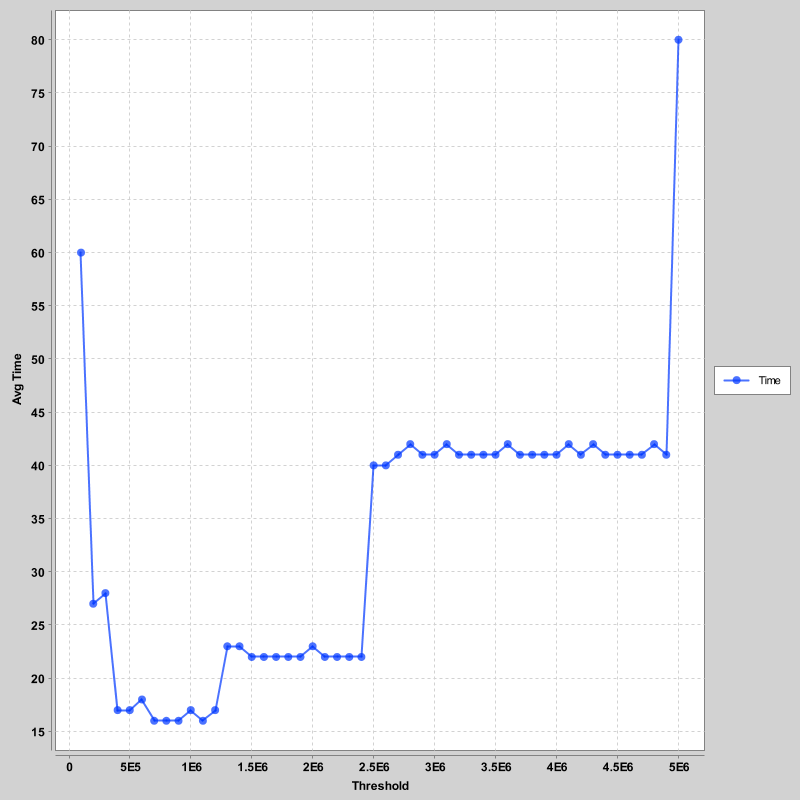
\includegraphics[width=\linewidth]{thres-vs-time-lighthouse.png}
  \caption{Lighthouse, Array size of 10000000, Time taken with no threading 157ms}
\endminipage\hfill
		\end{figure}		
	
		The graphs for Home PC 1, Laptop and Home PC 2 have the same trend of getting faster as the threshold gets higher (i.e. number of threads gets smaller). And in general ether perform better or just as good as the same sum computation performed without threading.\\
		
		The Lighthouse trend is more interesting as we see the fastest times are where the threshold is around $5*10^5$. As the threshold gets larger then the number of threads is less reducing the effectiveness of running such an algorithm on a machine like lighthouse.\\
	
		These results confirm what we previously found. Being that running such an algorithm performs exceptionally on a machine like lighthouse with a large number of CPU's otherwise we can only hope to achieve at best a little bit faster and at worse a lot slower than not using multi threading.
			
\end{document}